%!TEX root = ../main.tex
\section{Lab Activity 3}

This laboratory assignment requires to implement a robot that performs
phototaxis while avoiding collisions with obstacles. Once reached the black
spot under the light, it should halt. This set of behaviours should be
implemented by means of a \textbf{subsumption architecture}. A set of
``competences'' should then be defined, and place them in a hierarchical,
layered architecture.

\subsection{Designing the Subsumption Architecture}

The subsumption architecture is shown in \Cref{fig:sub-arch}. The layers are
placed in way that, when control is taken by an upper layer, it inhibits every
other underlying layer. Each layer can then use lower layers in order to
communicate or use the latter's information in order to implement higher-level
behaviours.
The \emph{competences} developed are the following (listed from lower to higher level):
%
\begin{figure}[ht]
    \centering
    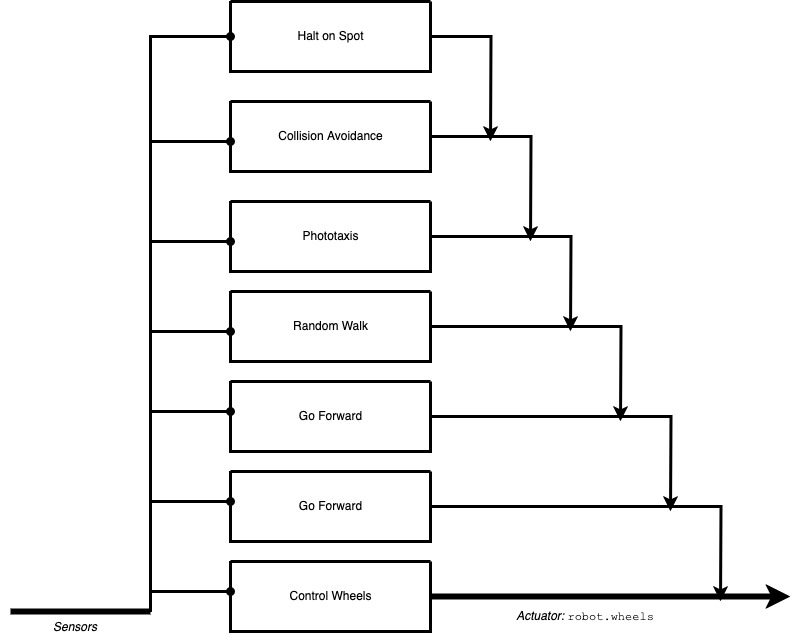
\includegraphics[width=0.6\textwidth]{figures/sub-arch.jpg}
    \caption{The Subsumption Architecture for archiving phototaxis while
        avoiding collisions and halting when under the light and over the black
        spot.}
    \label{fig:sub-arch}
\end{figure}
%
\begin{enumerate}
    \item \emph{Control Wheels} lets the definition of the simplest behaviour
        in order to control robot's wheels. It accepts a left and right
        velocities and sets the wheel velocities accordingly. It also avoid
        that the max speed of robot's wheels doesn't exceed $15^{-2}m/s$.
    \item \emph{Go Forward} defines a simple competence for moving forward,
        making use of its lower layer.
    \item \emph{Turn} accepts a direction on which the robot should turn to.
        Left or right turns are performed by multiplying current opposite wheel
        velocity by a factor (\texttt{TURN\_RATIO=3}) and the other wheel velocity by zero.
        This will let the robot to turn more gradually for finer turns.
    \item \emph{Random Walk} this competence performs a sub-optimal random walk by changing
        every $n$ steps robot wheels velocities randomly chosen.
    \item \emph{Follow Light}: phototaxis implementation. It picks maximum
        light value detected from sensors with the usual neighbour weighted
        average, and chose the direction to turn to based on which sensor
        yielded the maximum value.
    \item \emph{Avoid Front Obstacles}: collision avoidance implementation,
        with a difference that only front sensors are used for detecting
        collisions. If obstacles are detected, the controller checks collision
        for left, right and down, in this order. The first of these directions
        that does not contain an obstacle is used to perform a turn.
    \item \emph{Halt on Stop}: leveraging ground sensors, if any of those four
        detects that the robot is on the black spot, wheel velocities are set
        to zero.
\end{enumerate}
Having defined each layer and their dependencies, in order to keep the
``centralised'' piece of code as simple as possible, every layer makes use of a
shared boolean variable named \texttt{CONTROL\_TAKEN} which is reset at each
step. All layer includes the necessary checks for the shared variable before
performing their task. If they can take control, they set the variable to true,
if not, they early return.

With this approach we can archive coordination without complicating too much
the code, while keeping in mind that global state/variables can lead to
potential bugs and are sometimes discouraged. Another consideration that can be
made with shared variables in a distributed architecture like the subsumption
architecture, is that this can lead to race conditions, which can be easily
mitigated by means of mutex variables or atomic primitives (in this case an
atomic boolean).

\bigskip
With this approach, the control flow executes each layer in a top down fashion,
from the higher level to the lowest, and thanks to the shared state there is no
need of centralised coordination or inhibition by the main control flow.
